\documentclass[a4paper,12pt]{article}
\usepackage{latexsym, bbm, float}
\usepackage{amsmath}
\usepackage{amssymb}
\usepackage{amsthm}
\usepackage{graphicx}
\usepackage{fancyhdr}
\usepackage{type1cm}
%\usepackage{times}w
\usepackage{indentfirst}
\usepackage{makeidx}
\usepackage{amsfonts}
%\usepackage{wrapfigure}
\usepackage{hyperref}
\usepackage{color}
\usepackage{natbib}
\usepackage{listings}
% \usepackage{xcolor}
\usepackage{tabularx}
\usepackage{graphicx}
\usepackage{subfig}
\usepackage[normalem]{ulem}
\usepackage{times}
\usepackage{ulem}
\usepackage[dvipsnames]{xcolor}
% \usepackage[nocenter]{qtree}
% \usepackage{tree-dvips}
% \usepackage{gb4e}

\setlength{\oddsidemargin}{0.0in}
\setlength{\topmargin}{0.15in}
\setlength{\textwidth}{6.2in}
\setlength{\textheight}{8.75in}

\setlength{\parskip}{0.3cm}


\newcommand{\norm}[1]{\lVert#1\rVert}
\renewcommand{\baselinestretch}{1}
\pagenumbering{arabic}


\newtheorem{thm}{Theorem}[section]
\newtheorem{defn}{Definition}[section]
\newtheorem{lem}{Lemma}[section]
\newtheorem{cor}{Corollary}[section]
\newtheorem{assum}{Assumption}[section]


\theoremstyle{definition}
\newtheorem{exm}{Example}[section]
\newtheorem{remark}{Remark}[section]






%%%%%%%%%% define math symbols %%%%%%%%%%
%% bold and cal letters/LETTERS
\newcommand{\bfm}[1]{\ensuremath{\mathbf{#1}}}
\def\ba{\bfm a}     \def\bA{\bfm A}     \def\cA{{\cal  A}}     \def\calA{{\cal  A}}
\def\bb{\bfm b}     \def\bB{\bfm B}     \def\cB{{\cal  B}}     \def\calB{{\cal  B}}
\def\bc{\bfm c}     \def\bC{\bfm C}     \def\cC{{\cal  C}}     \def\calC{{\cal  C}}
\def\bd{\bfm d}     \def\bD{\bfm D}     \def\cD{{\cal  D}}     \def\calD{{\cal  D}}
\def\be{\bfm e}     \def\bE{\bfm E}     \def\cE{{\cal  E}}     \def\calE{{\cal  E}}
\def\bff{\bfm f}    \def\bF{\bfm F}     \def\cF{{\cal  F}}     \def\calF{{\cal  F}}
\def\bg{\bfm g}     \def\bG{\bfm G}     \def\cG{{\cal  G}}     \def\calG{{\cal  G}}
\def\bh{\bfm h}     \def\bH{\bfm H}     \def\cH{{\cal  H}}     \def\calH{{\cal  H}}
\def\bi{\bfm i}     \def\bI{\bfm I}     \def\cI{{\cal  I}}     \def\calI{{\cal  I}}
\def\bj{\bfm j}     \def\bJ{\bfm J}     \def\cJ{{\cal  J}}     \def\calJ{{\cal  J}}
\def\bk{\bfm k}     \def\bK{\bfm K}     \def\cK{{\cal  K}}     \def\calK{{\cal  K}}
\def\bl{\bfm l}     \def\bL{\bfm L}     \def\cL{{\cal  L}}     \def\calL{{\cal  L}}
\def\bm{\bfm m}     \def\bM{\bfm M}     \def\cM{{\cal  M}}     \def\calM{{\cal  M}}
\def\bn{\bfm n}     \def\bN{\bfm N}     \def\cN{{\cal  N}}     \def\calN{{\cal  N}}
\def\bo{\bfm o}     \def\bO{\bfm O}     \def\cO{{\cal  O}}     \def\calO{{\cal  O}}
\def\bp{\bfm p}     \def\bP{\bfm P}     \def\cP{{\cal  P}}     \def\calP{{\cal  P}}
\def\bq{\bfm q}     \def\bQ{\bfm Q}     \def\cQ{{\cal  Q}}     \def\calQ{{\cal  Q}}
\def\br{\bfm r}     \def\bR{\bfm R}     \def\cR{{\cal  R}}     \def\calR{{\cal  R}}
\def\bs{\bfm s}     \def\bS{\bfm S}     \def\cS{{\cal  S}}     \def\calS{{\cal  S}}
\def\bt{\bfm t}     \def\bT{\bfm T}     \def\cT{{\cal  T}}     \def\calT{{\cal  T}}
\def\bu{\bfm u}     \def\bU{\bfm U}     \def\cU{{\cal  U}}     \def\calU{{\cal  U}}
\def\bv{\bfm v}     \def\bV{\bfm V}     \def\cV{{\cal  V}}     \def\calV{{\cal  V}}
\def\bw{\bfm w}     \def\bW{\bfm W}     \def\cW{{\cal  W}}     \def\calW{{\cal  W}}
\def\bx{\bfm x}     \def\bX{\bfm X}     \def\cX{{\cal  X}}     \def\calX{{\cal  X}}
\def\by{\bfm y}     \def\bY{\bfm Y}     \def\cY{{\cal  Y}}     \def\calY{{\cal  Y}}
\def\bz{\bfm z}     \def\bZ{\bfm Z}     \def\cZ{{\cal  Z}}     \def\calZ{{\cal  Z}}
\def\bzero{\bfm 0}

% \boldsymbol{greek letters}
\newcommand{\bfsym}[1]{\ensuremath{\boldsymbol{#1}}}
\def \balpha   {\bfsym{\alpha}}       \def \bbeta    {\bfsym{\beta}}
\def \bgamma   {\bfsym{\gamma}}       \def \bdelta   {\bfsym{\delta}}
\def \bepsilon {\bfsym{\epsilon}}     \def \bzeta    {\bfsym{\zeta}}
\def \betta    {\bfsym{\eta}}         \def \btheta   {\bfsym{\theta}}
\def \biota    {\bfsym{\iota}}        \def \bkappa   {\bfsym{\kappa}}
\def \blambda  {\bfsym{\lambda}}      \def \bmu      {\bfsym{\mu}}
\def \bnu      {\bfsym{\nu}}          \def \bxi      {\bfsym{\xi}}
\def \bomicron {\bfsym{\omicron}}     \def \bpi      {\bfsym{\pi}}
\def \brho     {\bfsym{\rho}}         \def \bsigma   {\bfsym{\sigma}}
\def \btau     {\bfsym{\tau}}         \def \bupsilon {\bfsym{\upsilon}}
\def \bphi     {\bfsym{\phi}}         \def \bchi     {\bfsym{\chi}}
\def \bpsi     {\bfsym{\psi}}         \def \bomega   {\bfsym{\omega}}
\def \beps     {\bfsym \varepsilon}

% \boldsymbol{GREEK LETTERS}
\def \bGamma   {\bfsym{\Gamma}}       \def \bDelta   {\bfsym{\Delta}}
\def \bTheta   {\bfsym{\Theta}}       \def \bLambda  {\bfsym{\Lambda}}
\def \bXi      {\bfsym{\Xi}}          \def \bPi      {\bfsym{\Pi}}
\def \bSigma   {\bfsym{\Sigma}}       \def \bUpsilon {\bfsym{\Upsilon}}
\def \bPhi     {\bfsym{\Phi}}         \def \bPsi     {\bfsym{\Psi}}
\def \bOmega   {\bfsym{\Omega}}

% \hat{greek letters}
\renewcommand{\hat}{\widehat}
\def \halpha   {\hat{\alpha}}         \def \hbeta    {\hat{\beta}}
\def \hgamma   {\hat{\gamma}}         \def \hdelta   {\hat{\delta}}
\def \hepsilon {\hat{\epsilon}}       \def \hzeta    {\hat{\zeta}}
\def \heta     {\hat{\eta}}           \def \htheta   {\hat{\theta}}
\def \hiota    {\hat{\iota}}          \def \hkappa   {\hat{\kappa}}
\def \hlambda  {\hat{\lambda}}        \def \hmu      {\hat{\mu}}
\def \hnu      {\hat{\nu}}            \def \hxi      {\hat{\xi}}
\def \homicron {\hat{\omicron}}       \def \hpi      {\hat{\pi}}
\def \hrho     {\hat{\rho}}           \def \hsigma   {\hat{\sigma}}
\def \htau     {\hat{\tau}}           \def \hupsilon {\hat{\upsilon}}
\def \hphi     {\hat{\phi}}           \def \hchi     {\hat{\chi}}
\def \hpsi     {\hat{\psi}}           \def \homega   {\hat{\omega}}
\def \heps     {\hat{\heps}}

% \hat{\boldsymbol{greek letters}}
\def \hbalpha   {\hat{\balpha}}       \def \hbbeta    {\hat{\bbeta}}
\def \hbgamma   {\hat{\bgamma}}       \def \hbdelta   {\hat{\bdelta}}
\def \hbepsilon {\hat{\bepsilon}}     \def \hbzeta    {\hat{\bzeta}}
\def \hbeta     {\hat{\betta}}        \def \hbtheta   {\hat{\btheta}}
\def \hbiota    {\hat{\biota}}        \def \hbkappa   {\hat{\bkappa}}
\def \hblambda  {\hat{\blambda}}      \def \hbmu      {\hat{\bmu}}
\def \hbnu      {\hat{\bnu}}          \def \hbxi      {\hat{\bxi}}
\def \hbomicron {\hat{\bomicron}}     \def \hbpi      {\hat{\bpi}}
\def \hbrho     {\hat{\brho}}         \def \hbsigma   {\hat{\bsigma}}
\def \hbtau     {\hat{\btau}}         \def \hbupsilon {\hat{\bupsilon}}
\def \hbphi     {\hat{\bphi}}         \def \hbchi     {\hat{\bchi}}
\def \hbpsi     {\hat{\bpsi}}         \def \hbomega   {\hat{\bomega}}
\def \hbeps     {\hat{\beps}}

% \hat{\boldsymbol{GREEK LETTERS}}
\def \hbGamma   {\hat{\bGamma}}       \def \hbDelta   {\hat{\bDelta}}
\def \hbTheta   {\hat{\bTheta}}       \def \hbLambda  {\hat{\bLambda}}
\def \hbXi      {\hat{\bXi}}          \def \hbPi      {\hat{\bPi}}
\def \hbSigma   {\hat{\bSigma}}       \def \hbUpsilon {\hat{\bUpsilon}}
\def \hbPhi     {\hat{\bPhi}}         \def \hbPsi     {\hat{\bPsi}}
\def \hbOmega   {\hat{\bOmega}}


\newcommand{\lzeronorm}[1]{\lVert#1\rVert_0}
\newcommand{\lonenorm}[1]{\lVert#1\rVert_1}
\newcommand{\ltwonorm}[1]{\lVert#1\rVert_2}
\newcommand{\lfournorm}[1]{\lVert#1\rVert_4}
\newcommand{\opnorm}[1]{\lVert#1\rVert_{op}}
\newcommand{\fnorm}[1]{\lVert#1\rVert_F}
\newcommand{\nnorm}[1]{\lVert#1\rVert_N}
\newcommand{\supnorm}[1]{ \lVert#1  \rVert_{\max}}
\newcommand{\inn}[1]{\langle #1 \rangle}
\newcommand{\truncate}[1]{\sgn(#1)(|#1|\wedge \tau)}
\newcommand{\shrunk}[1]{#1 (\|#1\|_2 \wedge \tau)/\ltwonorm{#1}}
\newcommand{\shrunkt}[1]{#1^T \; (\|#1\|_2 \wedge \tau)/\ltwonorm{#1}}
\newcommand{\beq}  {\begin{equation}}
\newcommand{\eeq}  {\end{equation}}

\DeclareMathOperator*{\argmax}{argmax}
\DeclareMathOperator*{\argmin}{argmin}
\DeclareMathOperator{\corr}{corr}
\DeclareMathOperator{\cov}{cov}
\DeclareMathOperator{\Cov}{Cov}
\DeclareMathOperator{\Dev}{Dev}
\DeclareMathOperator{\diag}{diag}
\DeclareMathOperator{\E}{E}
\DeclareMathOperator{\logit}{logit}
\DeclareMathOperator{\rank}{rank}
\DeclareMathOperator{\RSS}{RSS}
\DeclareMathOperator{\sgn}{sgn}
\DeclareMathOperator{\supp}{supp}
\DeclareMathOperator{\Var}{Var}
\DeclareMathOperator{\var}{var}
\DeclareMathOperator{\SE}{SE}
\DeclareMathOperator{\tr}{tr}

\def \var   {\mbox{var}}
\def \corr  {\mbox{corr}}
\def \rase  {\mbox{RASE}}
\def \Cov   {\mbox{Cov}}
\def \C     {\mbox{const.}\quad}
\def \MSE   {\mbox{MSE}}
\def \MISE  {\mbox{MISE}}
\def \AMISE {\mbox{AMISE}}
\def \SE    {\mbox{SE}}
\def \se    {\mbox{SE}}
\def \andd  {\mbox{and}}
\def \logit {\mbox{logit}}
\def \new   {\mbox{new}}
\def \say   {\mbox{(say)}}
\def \MLE   {\mbox{\smallfont{MLE}}}
\def \U     {\mbox{\smallfont{U}}}
\def \sgn   {\mbox{sgn}}
\def \rcv   {{\rm RCV}}
\def \lasso {{\rm LASSO}}
\def \scad  {{\rm SCAD}}

\def \betaa    {\bbeta_{\alpha}^{\ast}}
\def \betas    {\bbeta^{\ast}}
\def \betah    {\bbeta_{\alpha}^{h}}
\def \betac    {\bbeta_{\alpha}^{c}}
\def \betacs   {\bbeta_{\alpha}^{c\ast}}
\def \sqLogpN  {\sqrt{(\log p)/n}}
\def \la       {\ell_{\alpha}}
\def \kl       {\kappa_{\cL}}
\def \ku       {\kappa_u}
\def \ko       {\kappa_0}
\def \Rd       {\mathbb{R}^d}
\def \Rdd	{\mathbb{R}^{d_1\times d_2}}
\def \RR	{\mathbb{R}}
\def \NN {\mathbb{N}}
\def \fd       {f_{\bDelta}}
\def \gd       {g_{\bDelta}}
\def \Rq       {R_{q}}
\def \bbP      {\mathbb{P}}
\def \bbS      {\mathbb{S}}
\def \sidx     {\sup_{(\bbeta,\bDelta)\in A'\cap \bDelta \in \bbS_1(\tau)}}
\def \vec	{\text{vec}}
\def \mat {\text{mat}}
\def \hcov	{\hat\Sigma^h_{yx_j}(\alpha)}
\def \ind {1}
\def \Tr {\text{Tr}}
\def \bbX {\mathbb{X}}
\def \bbY {\mathbb{Y}}
% Custom new command
\newcommand\redsout{\bgroup\markoverwith{\textcolor{red}{\rule[0.5ex]{2pt}{1pt}}}\ULon}

\title{COMS W 4111 Project 1 Progress Report}
\author{Xiaoyang Song (xs2485) \& Han Liu (hl3608)}
\date{UNI used to create schema: xs2485}

\begin{document}
\maketitle
\section{Modifications}
First of all, at this point, we do not change our applications and the functionalities that we introduced in proposal. However, after starting the implementation of data extraction and insertion, we made the following changes to our ER-Diagram and relational model schema, and add some real-world assumptions that we rely on:
\subsection{ER-Diagram}
\begin{enumerate}
    \item We \textcolor{Red}{\textbf{deleted}} the relationship set \textbf{Found} between entity set \textit{Inspection} and \textit{Violation}. We made this change because this relationship is redundant according to our ER-Diagram; in another word, removing this relationship set will not reduce any functionality of our model. As Professor Wu mentioned in lecture, everything that can be computed should not be included in the diagram. 
    
    The main reason we can remove this is that \textit{Inspection} and \textit{Violation} are indirectly related by \textit{Restaurants}; with that being said, we can perform everything between them by joining these three entity sets and the corresponding relationship sets together. \textbf{Found} is thus not necessary.
    \item We \textcolor{Green}{\textbf{added}} an attribute $v\_time$ for relationship set \textbf{Violate} to record when this violation happens. In our design, this is the same as its corresponding inspection time, which are recorded by $i\_time$ in \textbf{Inspect}. 
    \item Note that the name of attributes show up on the ER-Diagram may not be exactly the same as the one we used during implementation. This is because we want to make the ER-Diagram more informative while keep the implementation easy.
    % \item We \textcolor{Goldenrod}{\textbf{changed}} the constraints between \textit{Restaurant} and \textit{Location} to a \textit{Restaurant} can \textbf{locate} at at most one \textit{Location}. This enables the existence of a \textit{Restaurant} whose physical address is not recorded by the source data. We made this change because after manually inspecting the data, we discovered that the data of those \textit{Restaurants} whose addresses are not recorded might be useful for government staffs to analyze.
\end{enumerate}

\subsection{Relational Model Schema}
\begin{enumerate}
\item We \textcolor{Green}{\textbf{added}} a not null attribute and foreign key reference $lid$ to the schema of \textit{Restaurant} so that it can capture the exactly-one constraint precisely. Correspondingly, we \textcolor{Red}{\textbf{deleted}} the table \textbf{Locate} because we already include all information in table \textit{Restaurant}. However, we choose not to change the name of the relation \textit{Restaurant} when we combine them because this will make everything more informative.
    \item We \textcolor{NavyBlue}{\textbf{changed}} the primary key of relationship set \textbf{Inspect} to be tuple $(rid, iid, i\_time)$. We made this change because a \textit{Restaurant} can receive the same type of \textit{Inspection} for multiple times. However, our previous schema with only $(rid, iid)$ does not allow this. Adding inspection time into the primary key enable us to capture this property.
    \item Following exactly the same logic as for \textbf{Inspect}, we \textcolor{NavyBlue}{\textbf{changed}} the primary key of relationship set \textbf{Violate} to be tuple $(rid, vid, v\_time)$.
    \item Following exactly the same logic as for \textbf{Inspect}, we \textcolor{NavyBlue}{\textbf{changed}} the primary key of relationship set \textbf{Graded} to be tuple $(rid, gid, g\_time)$.
\end{enumerate}
\subsection{Assumptions}
When manually inspecting the source data and extracting/inserting them into database, we made the following assumptions, which are realistic and do not contradict with our design. \textcolor{Blue}{\textbf{Note that the assumptions that are made in project proposal still holds.}}
\begin{enumerate}
    \item A \textit{Restaurant} will not be \textbf{inspected} by the same \textit{Inspection} type twice at the same day.
    \item A \textit{Restaurant} will not be \textbf{graded} twice at the same day.
    \item A \textit{Restaurant} will not \textbf{violate} by the same \textit{Violation} twice at the same day.
    \item These three are just some template real-world assumptions that we tend to make for our project. More details will come out as we fully finish our implementations.
\end{enumerate}

\section{Partial Design Choice}
When extracting the data from source (.csv file) and insert them into the database, we found the following design choices useful and helpful for downstream tasks which we want to perform. Note that those choices do not violate our assumptions.
\begin{enumerate}
    \item For record with district not in NYC district set\footnotemark[1]\footnotetext[1]{NYC district sets = \{'Manhattan', 'Bronx', 'Brooklyn', 'Queens', 'Staten Island'\}}, we remove the record and do not insert them into databases. These are clear outliers. There is no need to deal with missing values because all records in source file have district information.
    \item For attributes in the tables which do not have not null constraints (i.e. optional attributes), if their values are not provided in the source data, we manually assign some informative values for them to indicate this fact. For example, $cuisine$ is an optional attribute in the table \textit{Restaurant}, when its value is not provided in the record, we put "No description is provided" to the table. Note that this is more informative than a NULL.
    \item For records whose restaurants acronym is not provided, we do not remove it and instead assign "Unknown" as their names. This prevents the information from being lost.
    \item When extracting grades data and insert them into table \textit{Grades} and \textbf{Graded}, we omit the grading records with missing $g\_time$; this is because grading time is crucial for our application and $g\_time$ is a part of the key of table \textbf{Graded}.
    \item More design choice will come out as we actually start implementing the web app.
\end{enumerate}
% \newpage
\section{ER-Diagram and Relational Model Schema}
Please refer to the Appendix for latest ER-Diagram and the CREATE TABLE code blocks.
\section{Populating Tables}
We implement the pipeline to extract data from source file and then automatically insert them into the database with edge case handling. Therefore, for this progress report, we extract 100 records (100/65499 rows in the source file) and insert them into databases for table \textit{Restaurant}, \textit{Locations}, \textit{Grade}, \textit{Inspection}, \textit{Violation}, \textbf{Graded}, \textbf{Violate}, and \textbf{Inspect}.

However, for tables \textit{Users}, \textit{Reviews\_Post\_Own}, and \textbf{Feel}, because we do not have records for them from source file, we  \textcolor{Blue}{\textbf{manually insert 10 or more records}} for each of them to illustrate the functionality of our database. \textcolor{Blue}{\textbf{In our design, these three tables will be gradually populated/updated as more \textit{Users} create accounts, share their feelings, and post reviews.}} For more details of data extraction/insertion and manual insertion procedure, please check \href{https://github.com/Xiaoyang-Song/NYC-Restaurant-Inspection-Database/blob/main/4111p1.ipynb}{here}. And all source codes for extraction and insertion can be found on \href{https://github.com/Xiaoyang-Song/NYC-Restaurant-Inspection-Database}{https://github.com/Xiaoyang-Song/NYC-Restaurant-Inspection-Database}.
\newpage
\section{Interesting Queries}
\begin{enumerate}
    \item Find the "Doing Business As" (i.e. $dba$) of Restaurants, along with their $rid$, that are in `Manhattan' and have rating level (i.e. $Grade$) of `A'. (no duplicates)
    \begin{verbatim}
    SELECT R.rid, R.dba
    FROM Restaurant AS R, Graded as GR, Grade as G
    WHERE R.rid=GR.rid AND GR.gid=G.gid AND G.grade='A'
    INTERSECT
    SELECT R.rid, R.dba
    FROM Restaurant AS R JOIN Locations as L on R.lid=L.lid
    WHERE L.district='Manhattan'
\end{verbatim}
\item Find the distribution of inspection types (i.e. $i\_type$), that is, find the total number of inspections for each inspection type. The final results should be ordered in descending order according to the total number of inspections for each type. The output of this query should be several rows with two columns ($i\_type$, count).
    \begin{verbatim}
    SELECT I.i_type, COUNT(*) AS count
    FROM Inspection as I, inspect AS IR, Restaurant AS R
    WHERE I.iid = IR.iid AND R.rid = IR.rid
    GROUP BY I.i_type
    ORDER BY COUNT(*) DESC
\end{verbatim}
\item Find the "Doing Business As" (i.e. $dba$) of restaurants, along with their $rid$ and total number of positive reviews, which have the highest number of positive reviews (assume there is no tie). For simplicity here, a review is positive if and only if it contains the word `good'. (We do not consider restaurant without reviews) The output of this query should be a single row with three columns.
    \begin{verbatim}
    SELECT R.rid, R.dba, COUNT(*)
    FROM Restaurant AS R, Reviews_Post_Own AS REV
    WHERE R.rid=REV.rid AND REV.content LIKE '%good%'
    GROUP BY R.rid, R.dba
    ORDER BY COUNT(*) DESC
    LIMIT 1
\end{verbatim}
\end{enumerate}
Note that these three queries are designed based on real-world applications. The detailed results can be found at the last section of  \href{https://github.com/Xiaoyang-Song/NYC-Restaurant-Inspection-Database/blob/main/4111p1.ipynb}{this notebook}. 

\newpage
\section{Appendix}
\subsection{ER-Diagram}
\begin{figure}[h]
    \centering
    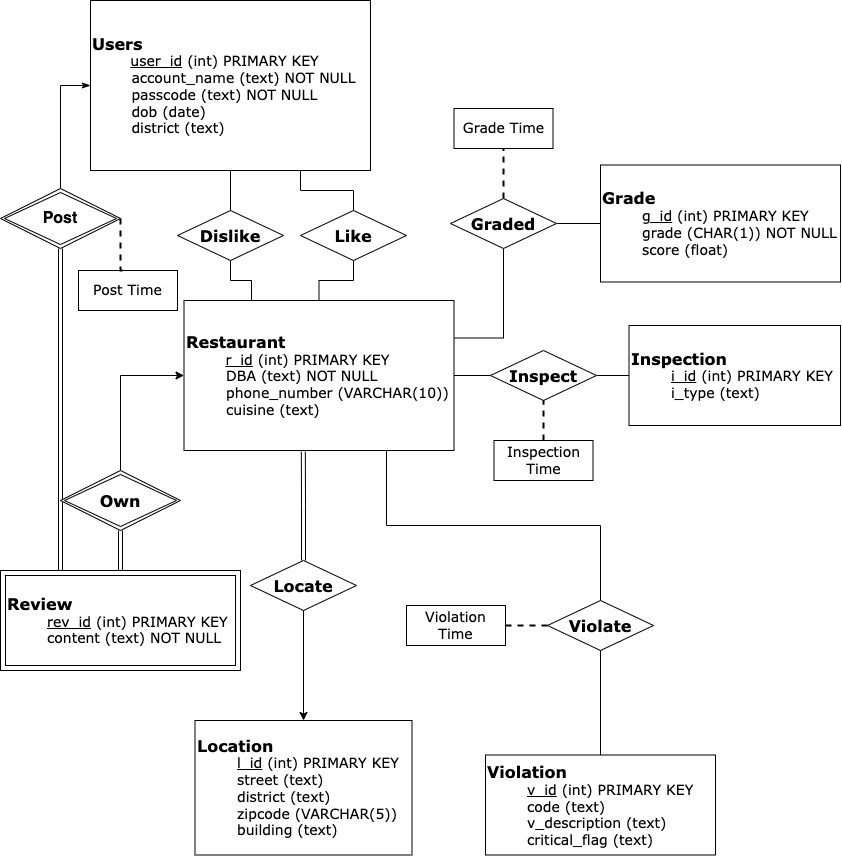
\includegraphics[scale=0.5]{Project1_ER.drawio.png}
    \caption{Latest ER-Diagram}
    \label{fig:er}
\end{figure}

\newpage
\subsection{CREATE TABLES}
\begin{verbatim}
-- Entity: Users
CREATE TABLE IF NOT EXISTS Users(
    userid serial PRIMARY KEY,
    account_name text NOT NULL,
    passcode text NOT NULL,
    dob date,
    district text,
    CHECK (
        district IN ('Manhattan', 'Bronx', 'Brooklyn', 
                     'Queens', 'Staten Island')
    )
);

-- Entity: Locations
CREATE TABLE IF NOT EXISTS Locations(
    lid serial PRIMARY KEY,
    district text,
    zipcode VARCHAR(5),
    street text,
    building text,
    CHECK (
        district IN ('Manhattan', 'Bronx', 'Brooklyn', 
        'Queens', 'Staten Island')
    )
);

-- Entity: Restaurant
-- Combine relationship sets and entity sets to model exactly-one
CREATE TABLE IF NOT EXISTS Restaurant(
    rid serial PRIMARY KEY,
    DBA text NOT NULL,
    phone_number VARCHAR(10), 
    cuisine text,
    lid int NOT NULL,
    FOREIGN KEY (lid) REFERENCES Locations
);

-- Entity: Grade
CREATE TABLE IF NOT EXISTS Grade(
    gid serial PRIMARY KEY,
    grade CHAR(1) NOT NULL,
    score float,
    CHECK (
        grade in ('A', 'B', 'C', 'P', 'N', 'Z')
    )
);

-- Entity: Inspection
CREATE TABLE IF NOT EXISTS Inspection(
    iid serial PRIMARY KEY,
    i_type text
);

-- Entity: Violation
CREATE TABLE IF NOT EXISTS Violation(
    vid serial PRIMARY KEY,
    code text,
    v_description text,
    critical_flag text,
    CHECK (
        critical_flag IN ('Critical', 'Not Critical', 
                          'Not Applicable')
    )
);

-- Combine relationship sets and entity sets to model weak entity
CREATE TABLE IF NOT EXISTS Reviews_Post_Own(
    rev_id serial PRIMARY KEY,
    content text NOT NULL,
    post_time DATE,
    userid int NOT NULL,
    rid int NOT NULL,
    FOREIGN KEY (userid) REFERENCES Users ON DELETE CASCADE,
    FOREIGN KEY (rid) REFERENCES Restaurant ON DELETE CASCADE
);

-- Relationship sets
-- note that when translating to relational schema
-- We combine Like and Dislike into Feel to make 
-- our design more efficient and elegant
CREATE TABLE IF NOT EXISTS Feel(
    userid int NOT NULL,
    rid int NOT NULL,
    feel text NOT NULL,
    PRIMARY KEY (userid, rid),
    FOREIGN KEY (userid) REFERENCES Users,
    FOREIGN KEY (rid) REFERENCES Restaurant,
    CHECK (
        feel IN ('Like', 'Dislike')
    )
);

-- Relationship set: Graded
CREATE TABLE IF NOT EXISTS Graded(
    rid int NOT NULL,
    gid int NOT NULL,
    g_time DATE NOT NULL,
    PRIMARY KEY (rid, gid, g_time),
    FOREIGN KEY (rid) REFERENCES Restaurant,
    FOREIGN KEY (gid) REFERENCES Grade
);

-- Relationship Set: Inspect
CREATE TABLE IF NOT EXISTS Inspect(
    rid int NOT NULL,
    iid int NOT NULL,
    i_time DATE NOT NULL,
    PRIMARY KEY (rid, iid, i_time),
    FOREIGN KEY (rid) REFERENCES Restaurant,
    FOREIGN KEY (iid) REFERENCES Inspection
);

-- Relationship Set: Violate
CREATE TABLE IF NOT EXISTS Violate(
    rid int NOT NULL,
    vid int NOT NULL,
    v_time DATE NOT NULL,
    PRIMARY KEY (rid, vid, v_time),
    FOREIGN KEY (rid) REFERENCES Restaurant,
    FOREIGN KEY (vid) REFERENCES Violation
);
\end{verbatim}
\end{document}
